\section{Silent Approximate Stores Protocol}

\begin{figure}[htbp]
	\centerline{\includegraphics[scale=0.4]{figures/MESI_SAS.pdf}}
	\caption{MESI SAS}
\label{fig:mesi_sas}
\end{figure}

Make a MESI coherence diagram showing how \textit{approximate stores} loop back into current state.

Explain each \textit{approx store} transitions

Maybe explain the two variants. One where you actually store the value, and one where you don't.